\chapter{Реализованная в симуляторе модель}

В этой главе описана реализованная в симуляторе модель. Это даст представление о том, как проходит процесс симуляции и какова степень подробности и точности симулятора.

\section{Многоагентное окружение с дискретным временем}

Основу симулятора представляет из себя многоагентая среда. Она состоит из агентов и ядра, которые общаются друг с другом посредством сообщений.

Ядро системы обеспечивает синхронизацию работы агентов и управляет временем. Симуляция не является непрерывной и разбита на дискретные единицы времени (ticks). Каждый tick соответствует одной минуте. Подобный выбор масштаба обуславливается тем, что предполагается достаточная скорость работы планировщика, чтобы успеть обработать запросы пришедшие в рамках одного tick'а за минуту. А исходя из того, что предполагаются довольно большие объемы датасетов, погрешность времени порядка минуты на передачу данных является допустимой.

\begin{figure}
	\centering
	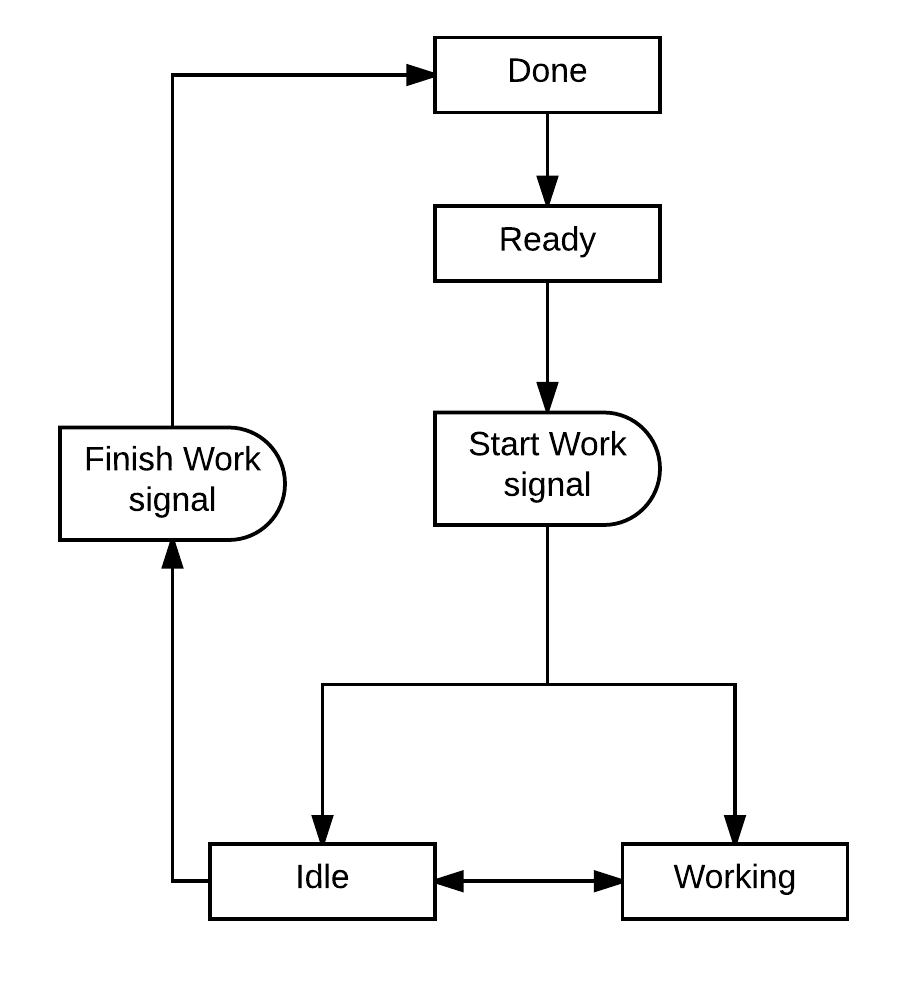
\includegraphics{fig/agent_workflow}
	\caption{Цикл работы агента}\label{fig:agent_workflow}
\end{figure}

В процессе каждого тика агент меняет свое состояние. Данный процесс цикличен. Возможные состояния агента и переходы между ними показаны на рисунке \ref{fig:agent_workflow}. Прямоугольники - это состояния. Второй тип элементов - это синхронизации. Синхронизация означает, что невозможно пройти по данному ребру, пока все агенты не будут готовы.

Описание состояний:

\begin{description}
	\item[Done] Означает, что предыдущий тик завершен успешно. Является исходным состоянием агента.
	\item[Ready] Означает, что агент готов начать работу в рамках нового тика.
	\item[Working] Означает, что агент в данный момент совершает работу.
	\item[Idle] Означает, что агент в данный момент бездействует и выполнил всю делегированную ему на данный момент работу.
\end{description}

Описание синхронизаций:

\begin{description}
	\item[Start Work] Дает гарантию, что перед началом работы все агенты достигли состояния Ready
	\item[Finish Work] Дает гарантию, что перед завершением тика все агенты находятся в состоянии Idle.
\end{description}

Важным аспектом является то, что признак завершения тика - это статус Idle у всех агентов системы. Это нужно помнить и не позволять системе попадать в это состояние, когда не вся работа сделана.

В состоянии Idle агент ждет одного из двух событий: новое сообщение от другого агента либо сигнал Finish Work. В последнем случае состояние меняется на Done. Эта смена состояния единственная не контролируется агентом напрямую.

Помимо основного статуса каждый агент имеет булев маркер stopFlag. Если он равен true, значит агент не запланировал никакой работы на будущие тики, и, если симуляция завершится сейчас, то это будет корректный исход.

Соответственно, симуляция завершается, когда у всех агентов stopFlag маркер равен true.

\section{Сетевое окружение}

В терминах описанной многоагентной среды симуляция сетевого окружения является заботой самих агентов. Причем это несложно реализуется: если агент знает свое место и места прочих агентов внутри сети, то он сам может накладывать ограничения на общения с этими агентами. То есть симуляция сети сводится к предоставлению конкретным агентам информации о конфигурации сети.

Структура сети в текущей версии симулятора представляет из себя набор из сегментов. Каждый сегмент содержит несколько машин. К одной машине могут быть привязаны один и более агентов.

Скорость передачи данных внутри сегмента и между сегментами может быть различной и является частью его описания.

\section{Параллелизм и коммуникация}

Агенты должны исполняться параллельно друг другу и ядру. Конечно, они могут блокировать друг друга - это соответствует ситуации, когда сервис не может ответить на новый запрос, пока не завершена обработка предыдущего. Но в рамках независимых участков кода мы получаем прирост производительности симуляции благодаря параллелизму. А в виду недетерминированного порядка выполнения этих участков - можем заметить состояния гонки вызванные недостаточно качественной проработкой архитектуры.

\section{Изоляция агентов}

В большинстве случаев агенты должны быть изолированы друг от друга. Это означает, что весь обмен информацией между ними должен происходить посредством сообщений.

В порядке исключения, конечно, можно использовать разделяемую память и мьютексы. Например, это годится для тех случаев, когда мы симулируем распределенное хранилище, а его конкретная реализация и возможность сбоев выходят за рамки эксперимента.

\section{Генерация сценариев}

Генерация сценариев, которые воспроизводятся в симуляции, должна происходить отдельно. Это позволит сравнивать поведение планировщиков и архитектуры в максимально приближенных условиях. Следовательно, симулятор должен предоставлять два инструмента: для генерации сценариев и для запуска симуляции.

Сценарий состоит из трех частей: конфигурация сети, описание датасетов и контейнеров, последовательность запросов в систему.

Сгенерированный сценарий представляет из себя набор YAML-файлов (вышеуказанные части лежат каждая в своем файле). При желании вместо генерации можно составить сценарий вручную или вносить правки в уже сгенерированный.

\section{Сбор статистики}

Нужно предоставить максимальную свободу в обработке данных. Это приводит к тому, что правильно сделать результатом работы симулятора логи, причем в удобном формате. В логи надо писать, что и когда произошло, а с помощью любого внешнего инструмента можно на основе логов выстроить произвольные метрики.

В данной работе в качестве формата логов был выбран JSON в виду хорошего баланса простоты и гибкости.

\section{Детали реализации компонентов системы}

Теперь подробнее рассмотрим принципы реализации конкретных компонентов архитектуры. Всего есть три типа агентов: Core, Control Unit, Worker

\subsection{Core}

Данный агент при инициализации получает список запросов. Каждому запросу из списка соответсвует порядковый номер тика, когда он должен быть послан в систему. Каждый отдельный запрос посылается случайному Control Unit'у.

\subsection{Control Unit}

К каждому Control Unit'у привязана группа Worker'ов. С данными Worker'ами может общаться только этот Control Unit.

В каждый момент времени ровно один Control Unit является лидером.

Control Unit содержит в себе следующий подкомпоненты:

\begin{description}
	\item[scheduler] - сам планировщик. Критически важна возможность использования одной и той же реализации планировщика как для симуляции, так и для реальных условий. Может либо пополнять очереди выполнения произвольных воркеров, либо делегировать запрос лидеру.
	\item[monitor] - компонент, который используется планировщиком, чтобы узнать глобальное состояние системы
	\item[local queue] - содержит очередь задач для подконтрольных воркеров. Компонент Executor из описания архитектуры в виду простоты своего устройства встроен в этот подкомпонент модели Control Unit.
\end{description}

Подкомпоненты работают в отдельных потоках выполнения.

Control Unit может принимать два типа запросов:

\begin{description}
	\item[Запросы на загрузку датасета или запуск контейнера c указанным датасетом] - данные запросы могут приходить от Core или быть делегированы другим Control Unit'ом. Обрабатываются scheduler'ом.
	\item[Запросы на добавление задачи в очередь подконтрольного Worker'а] - данные запросы приходят от других Control Unit'ов. Причина их появления в том, что при своей работе планировщик рассматривает все Worker'ы системы, а не только принадлежащие его Control Unit'у.
\end{description}

\subsection{Worker}

В один момент времени Worker может исполнять только один запрос. Запросы к нему могут приходить только от связанного с ним Control Unit'а.

Worker может принимать три вида запросов:

\begin{description}
	\item[Загрузка датасета] Время, необходимое на это, вычисляется на основе скорости передачи данных, полученной из описания сети.
	\item[Сборка контейнера] - в данный момент считается, что контейнер собирается за один тик. При желании этот параметр можно изменить.
	\item[Выполнение контейнера с заданным датасетом] - датасет и контейнер должны быть уже загружены на Worker. Время, необходимое на данную задачу, вычисляется по упрощенной модели: воркер имеет параметр производительности во флопсах, а контейнер имеет параметр, сколько флопс нужно на каждый мегабайт данных. Разделив одно на другое, получаем искомое время.
\end{description}